
Die üblichste Methode um eine Frequenzanalyse über ein längeres Signal anzuwenden ist die  Kurzzeit-Fourier-Transformation oder auch short-time Fourier transform, kurz STFT. Bei dieser Methode wird ein Signal, beschrieben durch $x(t)$, in kleine Zeitabschnitte zerhackt und bei jedem dieser Signalstücke eine Fourier-Transformation angwendet. Dabei wird üblicherweise die Fourier-Transformation in Anwendungen mit dem schnellen Fourier-Transformations Algorhytmus berechnet.\\

Wird nun ein Element der zerhackten Funktion $x(t)$ betrachtet kann der Start- und Endwert beliebig sein. Diese Sprünge haben bekanntlich Folgen, die im Frequenzbereich ersichtlich werden können durch eine Verschmierung über die Frequenzen auch Unschärfe genannt. \\

Um dies zu verdeutlichen wird in der Abbildung \ref{fig:Spectral} ein unendlich langes Signal $x(t)=sin(t)$ untersucht. 
\begin{figure}[!ht]
	\centering
	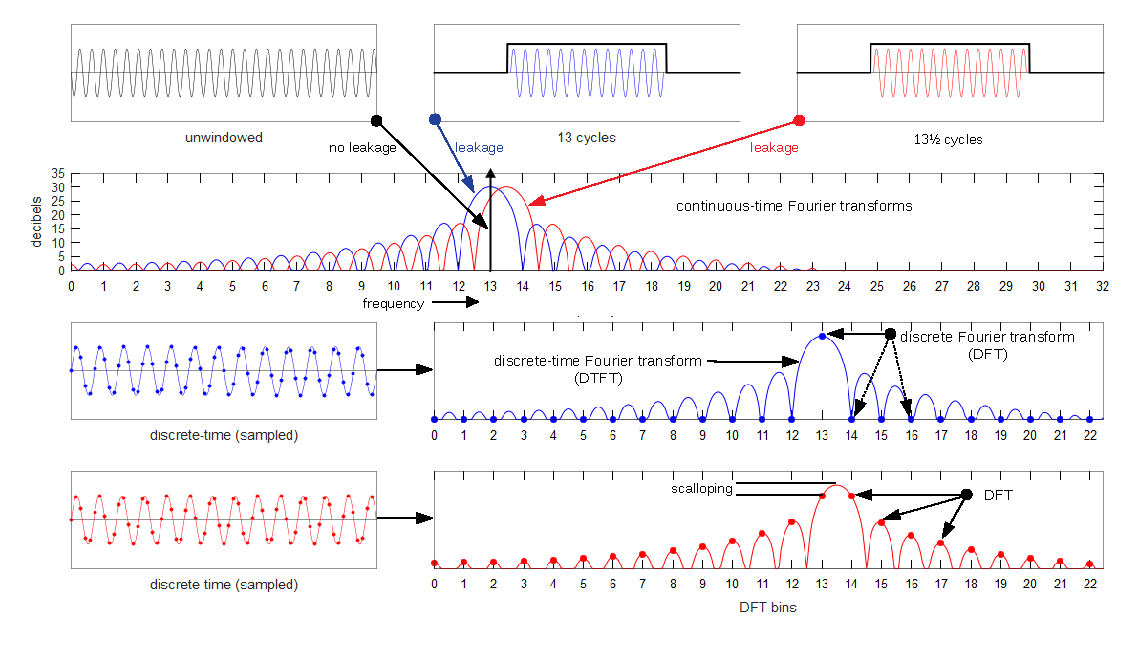
\includegraphics[scale=0.8]{papers/autotune/sections/fft/images/windows/Spectral.pdf}
	\caption{Darstellung der Fensterung und dessen mögliche Frequenzverschmierung/Unschärfe}\cite{wikipedia:Window}
	\label{fig:Spectral}
\end{figure}%

Zuerst werden die Signale Zeitkontinuierlich berachtet. Im ersten Beispiel in \ref{fig:Spectral} wird das unendliche kontinuierliche Signal $x(t)$ schwarz im Frequenzbereich abgebildet. Dieses Resultat ist scharf und zeigt und genau eine Frequenz.\\

Beim zweiten Beispiel in \ref{fig:Spectral} (in Blau) wird das Signal $x(t)$ mit der Fensterfunktion $w_{1}(t)$ multipliziert.\\
Wobei gilt: 
\begin{equation}
	w_{1}(t)= \left\{\begin{array}{lll}{t<\alpha,} & {0} \\ {\alpha\leq t \leq\beta_{1},} & {1}\\ {t>\beta_{1},}&{0}\end{array}\right\}
\end{equation}
\begin{equation}
	\hat{f_{1}}(\omega)=\frac{1}{\sqrt{2 \pi}} \int_{-\infty}^{\infty} w_{1}(t)\cdot f(t) \cdot e^{-\mathrm{i} \omega t} \mathrm{d} t
\end{equation}

$\alpha$ und $\beta_{1}$ decken ein Zeitintervall von $13$ Perioden ab. Im Frequenzbereich ist nun in Blau ersichtlich das die Fourier-Transformation im eine deutliche Unschärfe zur Folge hat welche im Kontinuierlichen Spektrum ersichtlich wird. Das Maxima der Amplitude korreliert mit dem Frequenzvektor des Originalen Signales $x(t)$\\




Im letzten Fall in \ref{fig:Spectral} wird $x(t)$ mit der Fensterfunktion $w_{2}(t)$ multipliziert.\\
Wobei gilt: 
\begin{equation}
	w_{2}(t)= \left\{\begin{array}{lll}{t<\alpha,} & {0} \\ {\alpha\leq t \leq\beta_{2},} & {1}\\ {t>\beta_{2},}&{0}\end{array}\right\}
\end{equation}
\begin{equation}
	\hat{f_{2}}(\omega)=\frac{1}{\sqrt{2 \pi}} \int_{-\infty}^{\infty} w_{2}(t)\cdot f(t) \cdot e^{-\mathrm{i} \omega t} \mathrm{d} t
\end{equation}

Wobei $\alpha$ und $\beta_{2}$ ein Zeitintervall von $13\frac{1}{2}$ Perioden abdecken. Nun sieht man nicht nur eine Unschärfe sondern auch eine fehlende Korrelation zwischen dem Maxima und der eigentlichen Frequenz des Signales $x(t)$.\\
Betrachtet man nun die Diskreten Punkte der beiden mit einem Fenster belegten Signalen entdeckt man erstaundliches. Ist das Signal genau über über ein vielfaches der Periode gefenstert ist im diskreten Fall keine Frequenzunschärfe erkennbar. Trifft es jedoch auf eine zufällige Stelle im Signal und deckt nicht gerade eine Periode ab zeigen die Diskreten ein nur schwer zu interpretierbares Ergebnis an. Man spricht von einer Unschärfe die da nicht die eigentliche Frequenz des Signales $x(t)$ abgebildet wird sondern ein ganzes Band.\\
Versucht man nun ein reales Signal zu Analysieren die meistens nicht periodisch auftreten und mit diskreten Werten beschrieben ist diese Unschärfe meistens gegeben. Nun gibt es verschiedenste Methoden um diese Frequenzanalyse zu realisieren. In diesem Paper wird jedoch nur auf die Short Fourrier-Transformation und die Wavelet-Transformation eingegangen. 


\subsection{Zeitkontinuierliche STFT}

Das Produkt des Signals $x(t)$ mit der Fensterfunktion $w(t) $ liefert uns also eine neue Funktion die im Bereich ausserhalb des Fensters alle Werte auf null gesetzt hat. In der Anwendung sind diese Fenster meistens ein wenig überlappend damit kein Datenverlust entsteht. \\
Die Zeitkontiunierliche STFT ist  gegeben als:
\begin{equation}
	\hat{f}(\tau, \omega)=\int_{-\infty}^{\infty} x(t)\cdot w(t-\tau)\cdot e^{-j \omega t} dt
\end{equation}
mit der Kreisfrequenz  $\omega $

\subsection{Zeitdiskrete STFT}
Bei der Zeitdiskreten STFT liegt das Signal in einzelnen Abtastwerten vor. Diese Abtastwerte werden dann durch die Fensterfunktionen in einzelne Abschnitte unterteilt. \\
Die diskrete STFT ist gegeben als:
\begin{equation}
	\hat{f}(m, \omega)=\sum_{n=-\infty}^{\infty} x_{n} \cdot w_{n-m}\cdot e^{-j \omega n}
\end{equation}


\subsection{Fensterfunktionen}
Um die Unschärfe Problematik der STFT zu verbessern gibt es eine ganze Reihe an verschiedenen Fensterfunktionen die verwendet werden können um ein besseres Resultat zu erreichen. Die Auswahl der Funktion ist dabei Anwendungsspezifisch. In der Folgenden Tabelle \ref{tab:STFTtab} findet man eine kleine Auswahl mit dem jeweiligen Spektrum 


\begin{figure}[!ht]
	\begin{minipage}{.4\columnwidth}
		\textbf{Rechteck-Fenster}\\
		$w_{n}=1$
	\end{minipage}%
	\begin{minipage}{.6\columnwidth}
		\centering
		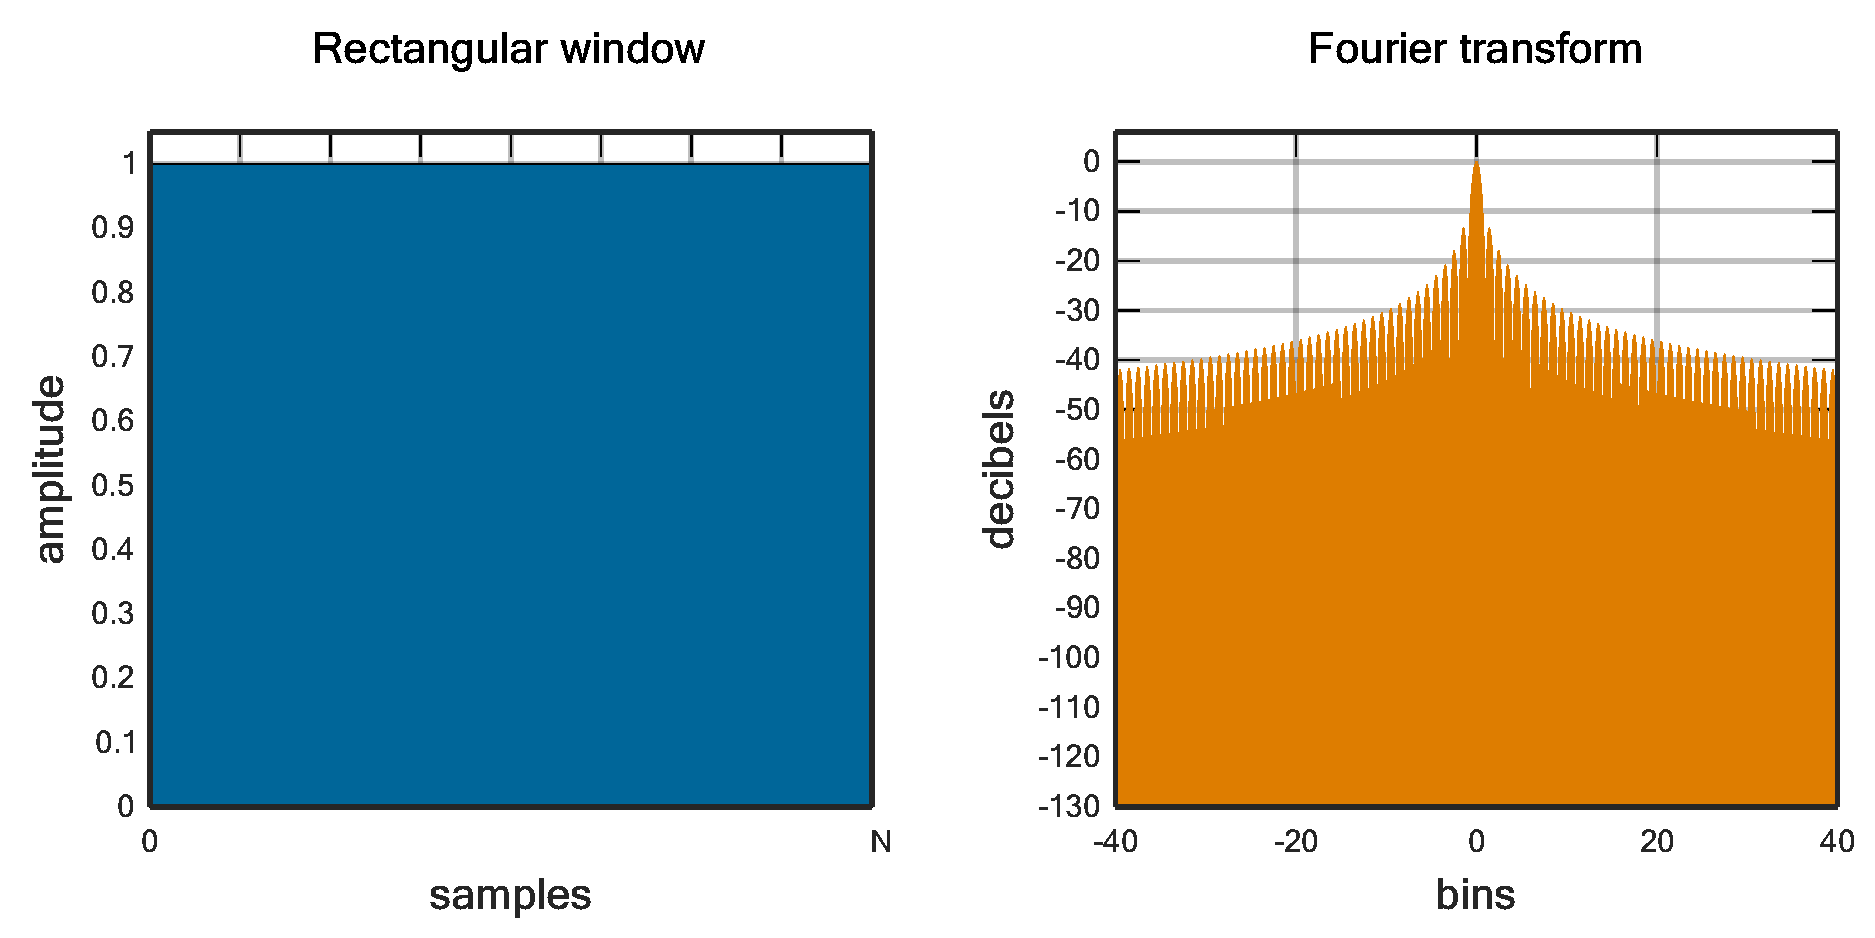
\includegraphics[width=\linewidth]{papers/autotune/sections/fft/images/windows/Rectangular.pdf}
	\end{minipage}


	\begin{minipage}{.4\columnwidth}
		\textbf{Gauss-Fenster} mit $\sigma = 0.4$\\
		$w_{n}=e^{-\frac{1}{2}\left(\frac{n-N / 2}{\sigma N / 2}\right)^{2}},$\\
		$ \quad 0 \leq n \leq N$\\
		$\sigma \leq 0.5$
	\end{minipage}%
	\begin{minipage}{.6\columnwidth}
		\centering
		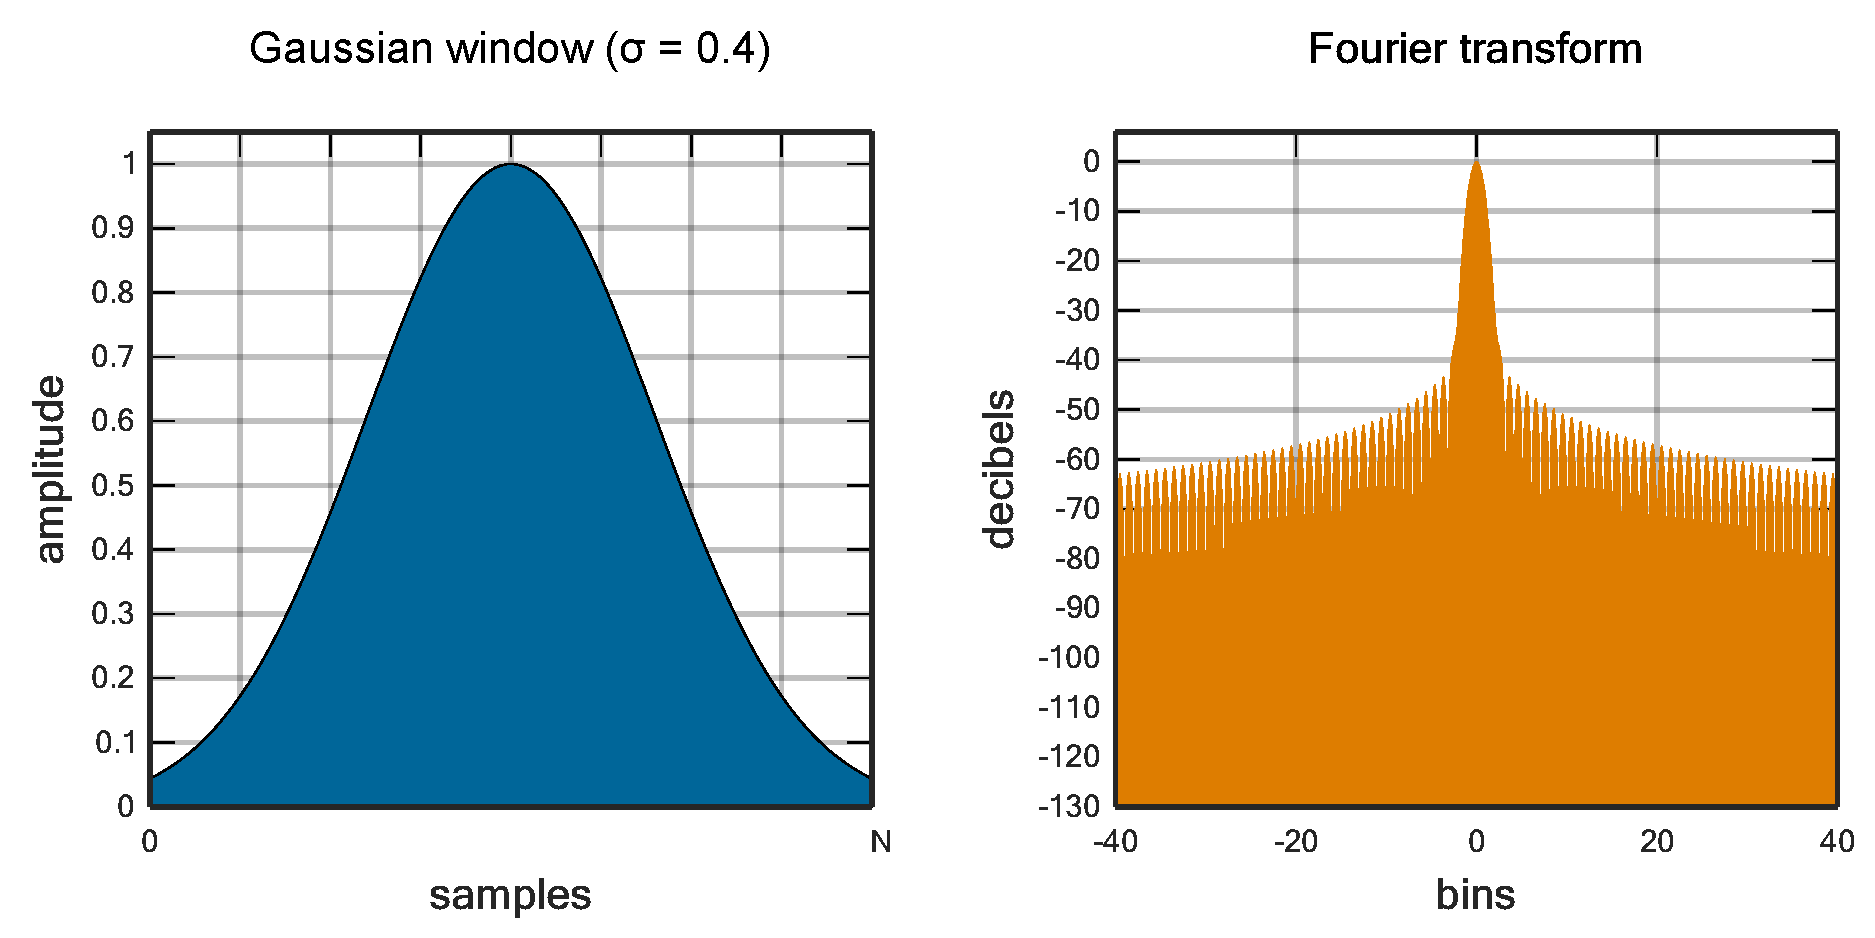
\includegraphics[width=\linewidth]{papers/autotune/sections/fft/images/windows/Gauss.pdf}
	\end{minipage}


	\begin{minipage}{.4\columnwidth}
		\textbf{Blackman-Fenster}\\
		$\begin{array}{l}{w_{n}=a_{0}-a_{1} \cos \left(\frac{2 \pi n}{N}\right)+a_{2} \cos \left(\frac{4 \pi n}{N}\right)} \\ 		{a_{0}=\frac{1-\alpha}{2} ; \quad a_{1}=\frac{1}{2} ; \quad a_{2}=\frac{\alpha}{2}}\end{array}$
	\end{minipage}%
	\begin{minipage}{.6\columnwidth}
		\centering
		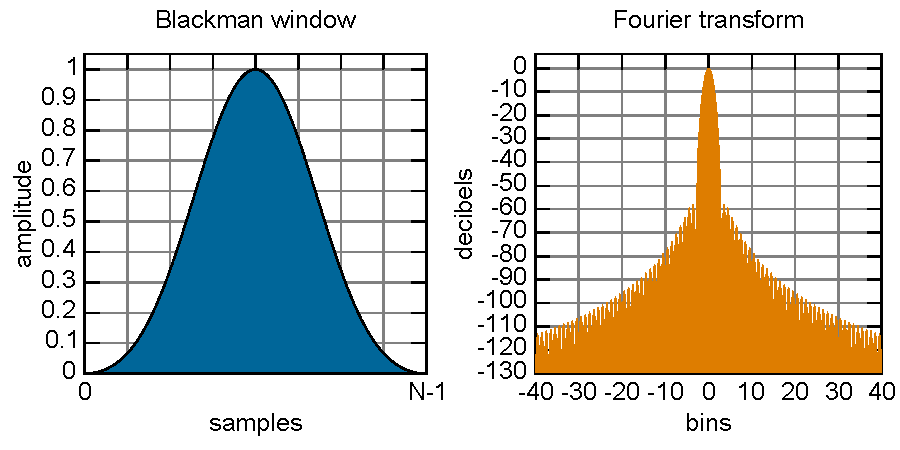
\includegraphics[width=\linewidth]{papers/autotune/sections/fft/images/windows/Blackman.pdf}
	\end{minipage}


	\begin{minipage}{.4\columnwidth}
		\textbf{Blackman-Harris-Fenster}\\
		$w_{n}=a_{0}-a_{1} \cos \left(\frac{2 \pi n}{N}\right)+a_{2} \cos \left(\frac{4 \pi n}{N}\right)-a_{3} \cos \left(\frac{6 \pi n}{N}\right)$\\
		wobei:
		$a_{0}=0.35875 ; \quad a_{1}=0.48829 ;$\\
		$ \quad a_{2}=0.14128 ; \quad a_{3}=0.01168$
	\end{minipage}%
	\begin{minipage}{.6\columnwidth}
		\centering
		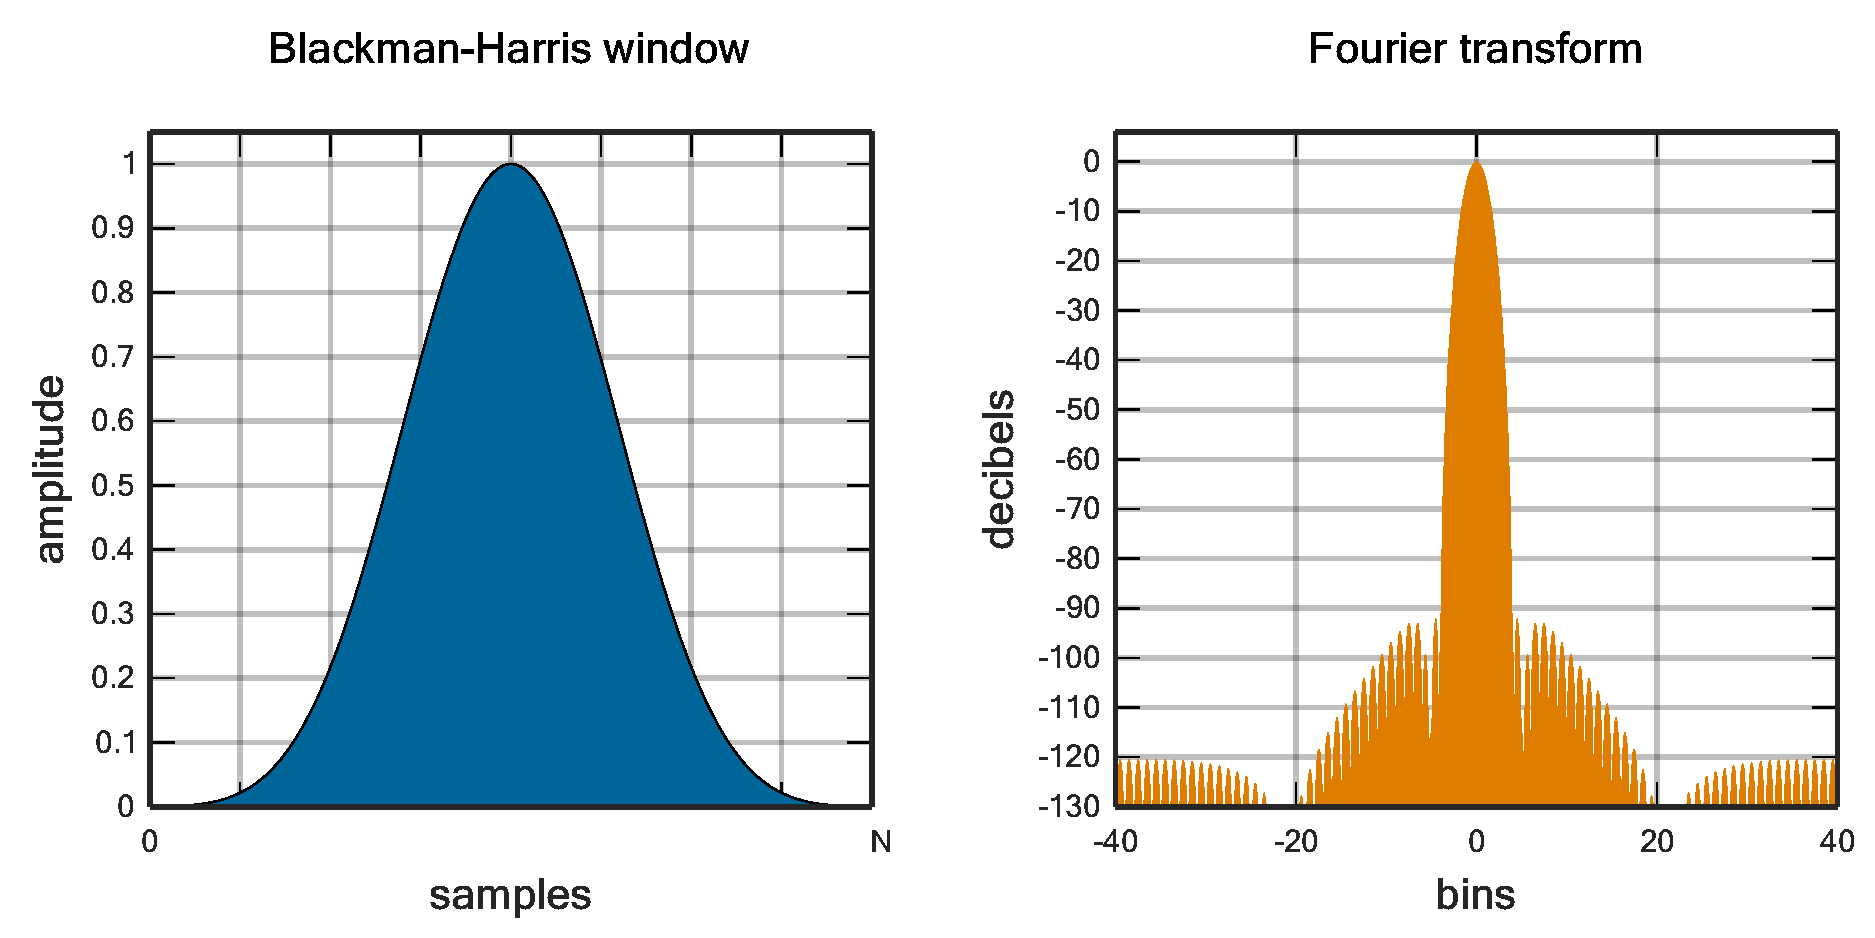
\includegraphics[width=\linewidth]{papers/autotune/sections/fft/images/windows/Blackman-Harris.pdf}
	\end{minipage}

\caption{Verschiedene Fensterfunktionen und deren Beschreibung}\cite{wikipedia:Window}
\label{fig:STFTtab}
\end{figure}



\subsection{Verhalten der STFT}

Wenn man ein Signal mit einer Fensterfunktion Analysiert, zerteilt man das Signal in der Zeitebene vertikal Streifen mit der Breite eines Fensterintervalles. Wendet man nun darauf noch die Fourier-Transformation an wird jeder Streifen in rechtecke aufgeteilt. Die höhe des Rechteckes wird durch die Unschärferelation bestimmt. Daraus folgt bei einem breiteren Streifen ergibt sich eine besser Frequenzauflösung, was jedoch einen schlechtere Zeitauflösung bedeutet. In der Abbildung \ref{fig:stftauf} kann man die grafische Darstellung der Zeit-Frequenz-Auflösung sehen. Bei gleichbleibendem Flächeninhalt der einzelnen Rechtecke ist auf der linken Seite eine feinere Zeitauflösung zu sehen. Wobei Rechts eine bessere Frequenzauflösung aufweist. Dies wird durch die Küpfmüllerschen Unbestimmtheitsrelation welche besagt, dass die Zeitdauer und die Bandbreite eines Signals nicht gleichzeitig beliebig klein werden können. Dies ist eine zur Heisenbergschen Unschärferelation analoge Aussage welche auf die Nachrichtentechnik übernommen werden kann.

\begin{figure}[!ht]
	\centering
	\scalebox{.75}{
	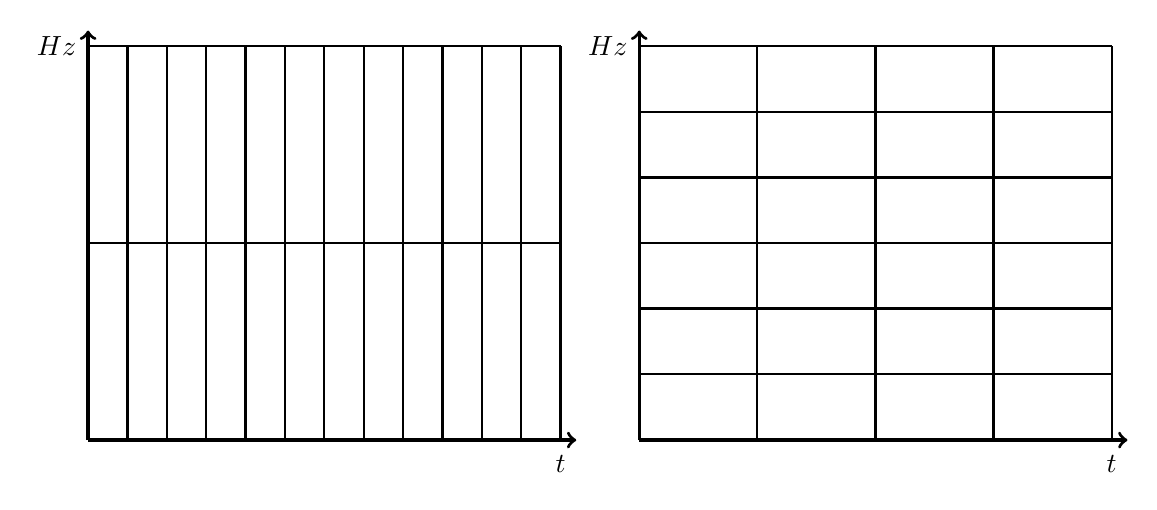
\begin{tikzpicture}
		\draw (6,-5.3) node{$t$};
		\draw (-0.4,0) node{$Hz$};
		\draw[->, very thick] (0,-5)--(0,0.2);
		\draw[->, very thick] (0,-5)--(6.2,-5);
		
		\draw[thick] (0,-0)--(6,-0);
		\draw[thick] (0,-2.5)--(6,-2.5);
		
		\draw[thick] (0.5,-5)--(0.5,0);
		\draw[thick] (1,-5)--(1,0);
		\draw[thick] (1.5,-5)--(1.5,0);
		\draw[thick] (2,-5)--(2,0);
		\draw[thick] (2.5,-5)--(2.5,0);
		\draw[thick] (3,-5)--(3,0);
		\draw[thick] (3.5,-5)--(3.5,0);
		\draw[thick] (4,-5)--(4,0);
		\draw[thick] (4.5,-5)--(4.5,0);
		\draw[thick] (5,-5)--(5,0);
		\draw[thick] (5.5,-5)--(5.5,0);
		\draw[thick] (6,-5)--(6,0);
		
		\draw (13,-5.3) node{$t$};
		\draw (6.6,0) node{$Hz$};
		\draw[->, very thick] (7,-5)--(7,0.2);
		\draw[->, very thick] (7,-5)--(13.2,-5);
		
		\draw[thick] (7,-0)--(13,-0);
		\draw[thick] (7,-0.833)--(13,-0.833);
		\draw[thick] (7,-1.666)--(13,-1.666);
		\draw[thick] (7,-2.499)--(13,-2.499);
		\draw[thick] (7,-3.33)--(13,-3.33);
		\draw[thick] (7,-4.166)--(13,-4.166);
		
		\draw[thick] (8.5,-5)--(8.5,0);
		\draw[thick] (10,-5)--(10,0);
		\draw[thick] (11.5,-5)--(11.5,0);
		\draw[thick] (13,-5)--(13,0);
	\end{tikzpicture}
	}
	\caption{STFT Zeit-Frequenz-Auflösung}\label{fig:stftauf}	
\end{figure}

\begin{figure}[!ht]
	\centering
	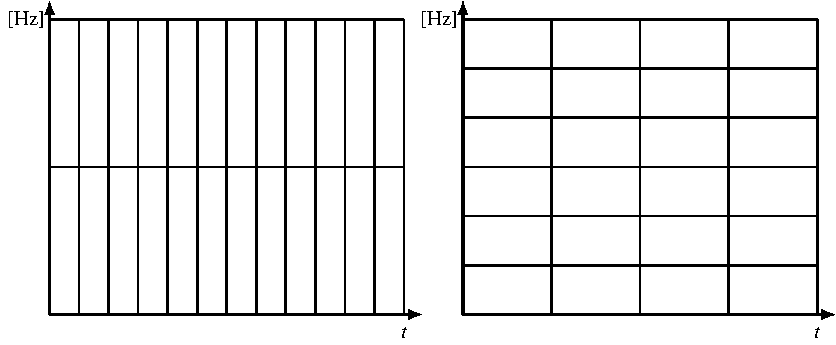
\includegraphics[width=0.7\linewidth]{papers/autotune/sections/fft/images/windows.pdf}
	\caption{STFT Zeit-Frequenz-Auflösung}\label{fig:stftauf}	
\end{figure}





 
Um das zu veranschaulichen  der Unschärferelation betrachten wir einen modulierten Frequensweep von 0 bis 400$[Hz]$. Die Definition der verwendeten Frequenzsweepes $x_{sweep}(t)$ ist folgendermassen:

\begin{equation}
x_{sweep}(t)=\sin \left(2 \pi \int_{0}^{t} f(\tau) \mathrm{d} \tau\right)=\sin \left(2 \pi \int_{0}^{t}\left(f_{0}+k \tau\right) \mathrm{d} \tau\right)=\sin \left(2 \pi\left(f_{0}+\frac{k}{2} t\right) t\right)
\end{equation} 

Der Sweep wird nun mit einem viel langsameren Signal, welches aus einem verschobenen Cosinus besteht, moduliert. Die Defenition des zu Analysierende Signales $f(t)$ lautet dementsprechend:
\begin{equation}
f(t)= (-0.5\cdot \cos(nt)+0.5)\cdot x(t)=(-0.5\cdot \cos(nt)+0.5)\cdot \sin \left(2 \pi \int_{0}^{t} f(\tau) \mathrm{d} \tau\right)
\end{equation} \label{eq:sin-sweep}
wobei $n$ die Anzahl von Perioden des Cosinus in einer Zeit von $2\pi$ ist. Danach wurde $f(t)$ mit dem STFT Verfahren analysiert. Insgesamt wurde $f(t)$ vier mal analysiert. Jede Analyse wurde mit der Blackman Fensterfunktion durchgeführt jedoch wurden die Fenster in ihrer Breite verändert. Diese Veränderung trägt zu dem Verständnis der Unschärferelation bei. Die verwendete Blackmanfunktion ist in der Tabelle \ref{tab:STFTtab} definiert.\\

In der Grafik \ref{fig:STFT} kann nun diese Unschärferaltion beobachtet werden. Die Unschärfe wird gut erkennbar wenn man ein beliebiges Signal mit zeitlich verschieden langen Fenstern Analysiert. Wobei bei diskreten werten dies direkt in anzahl Samples pro Fenster gesehen werden muss.\\



\begin{figure}[!ht]
	\centering
	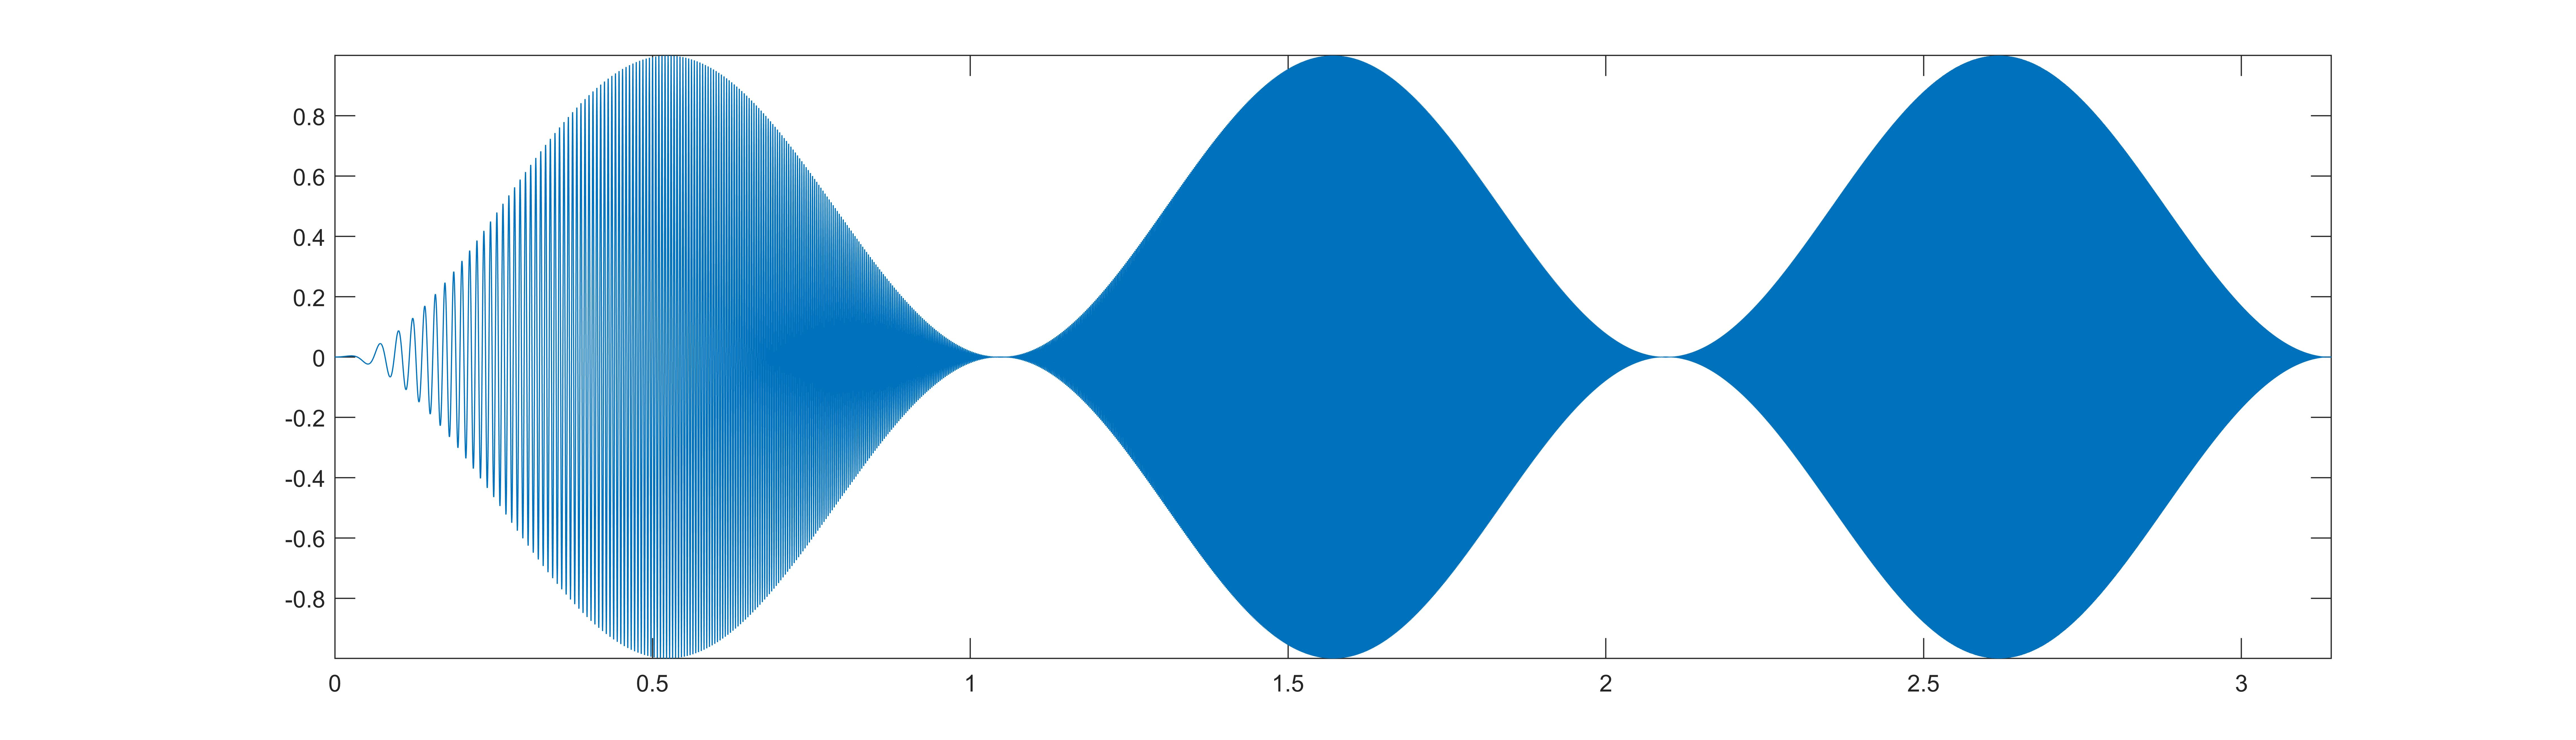
\includegraphics[width=\linewidth]{papers/autotune/sections/fft/signal.jpg}
	\captionof{figure}{Sweep Signal 0-400$Hz$}\label{fig:stftsig}
	\begin{tabularx}{\columnwidth}{XX}
		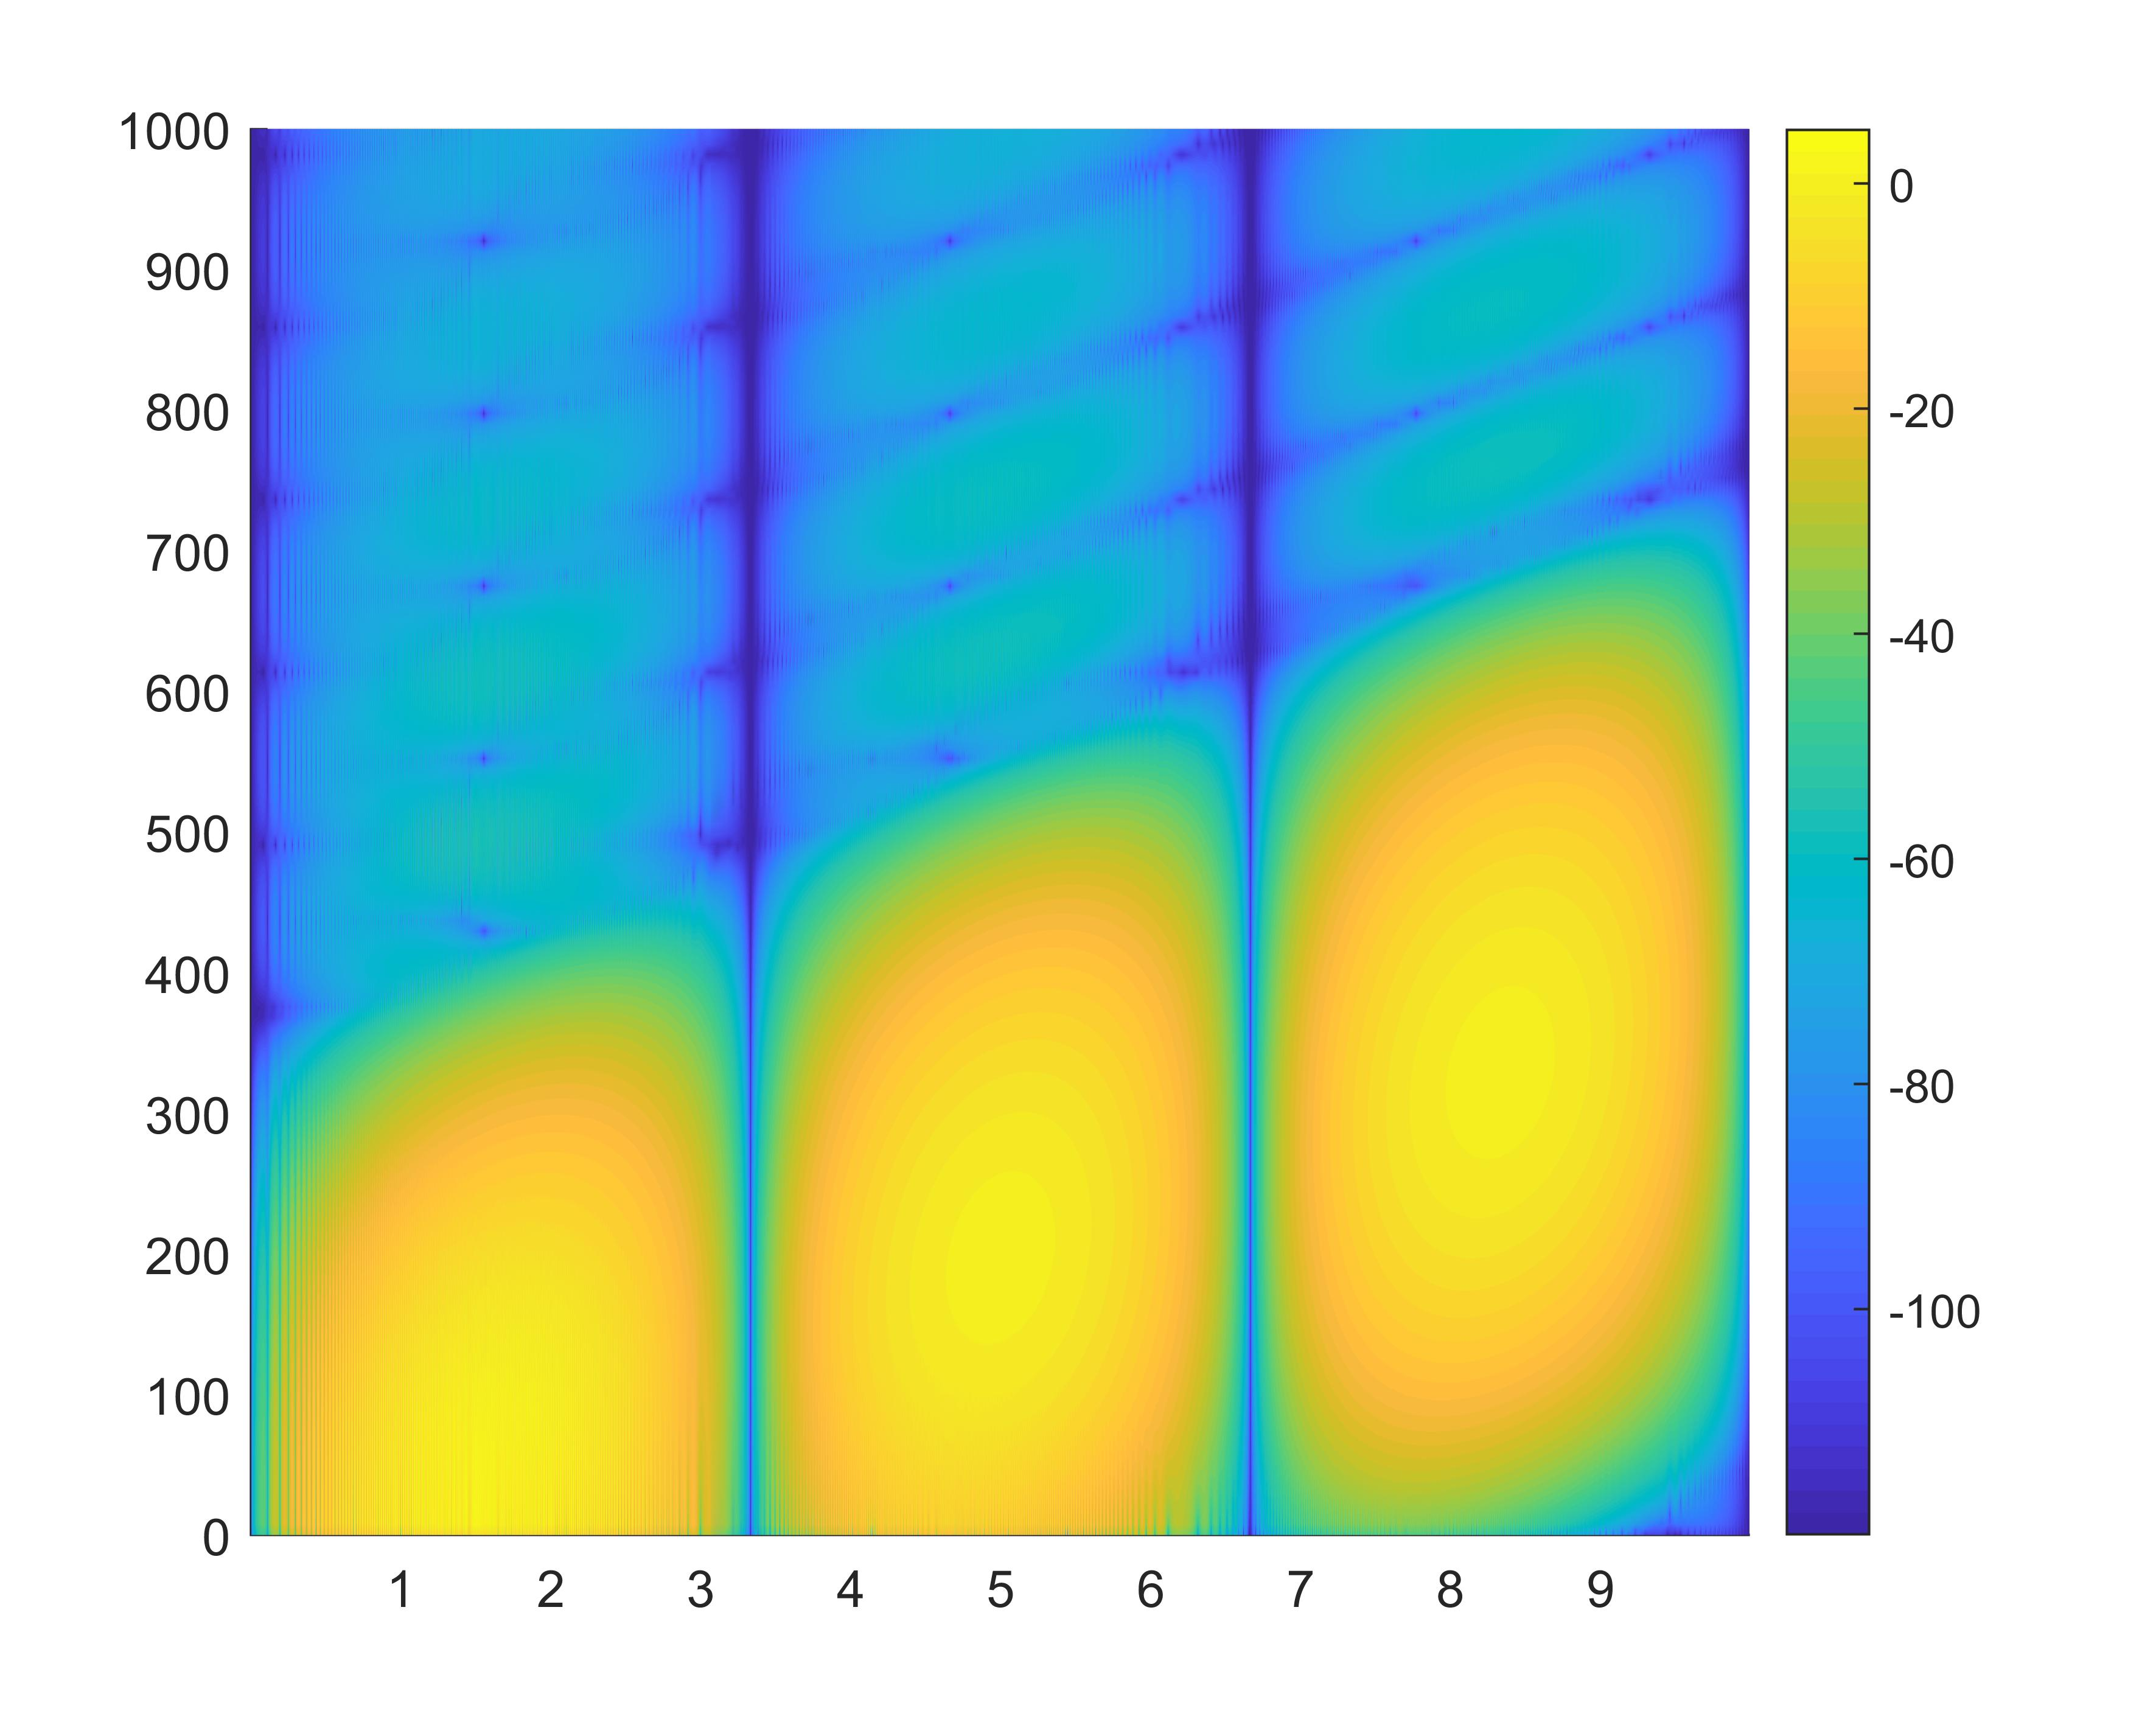
\includegraphics[width=\linewidth]{papers/autotune/sections/fft/stft256.jpg}
		\captionof{figure}{256 Sample Fenster}\label{fig:stft256}
		&   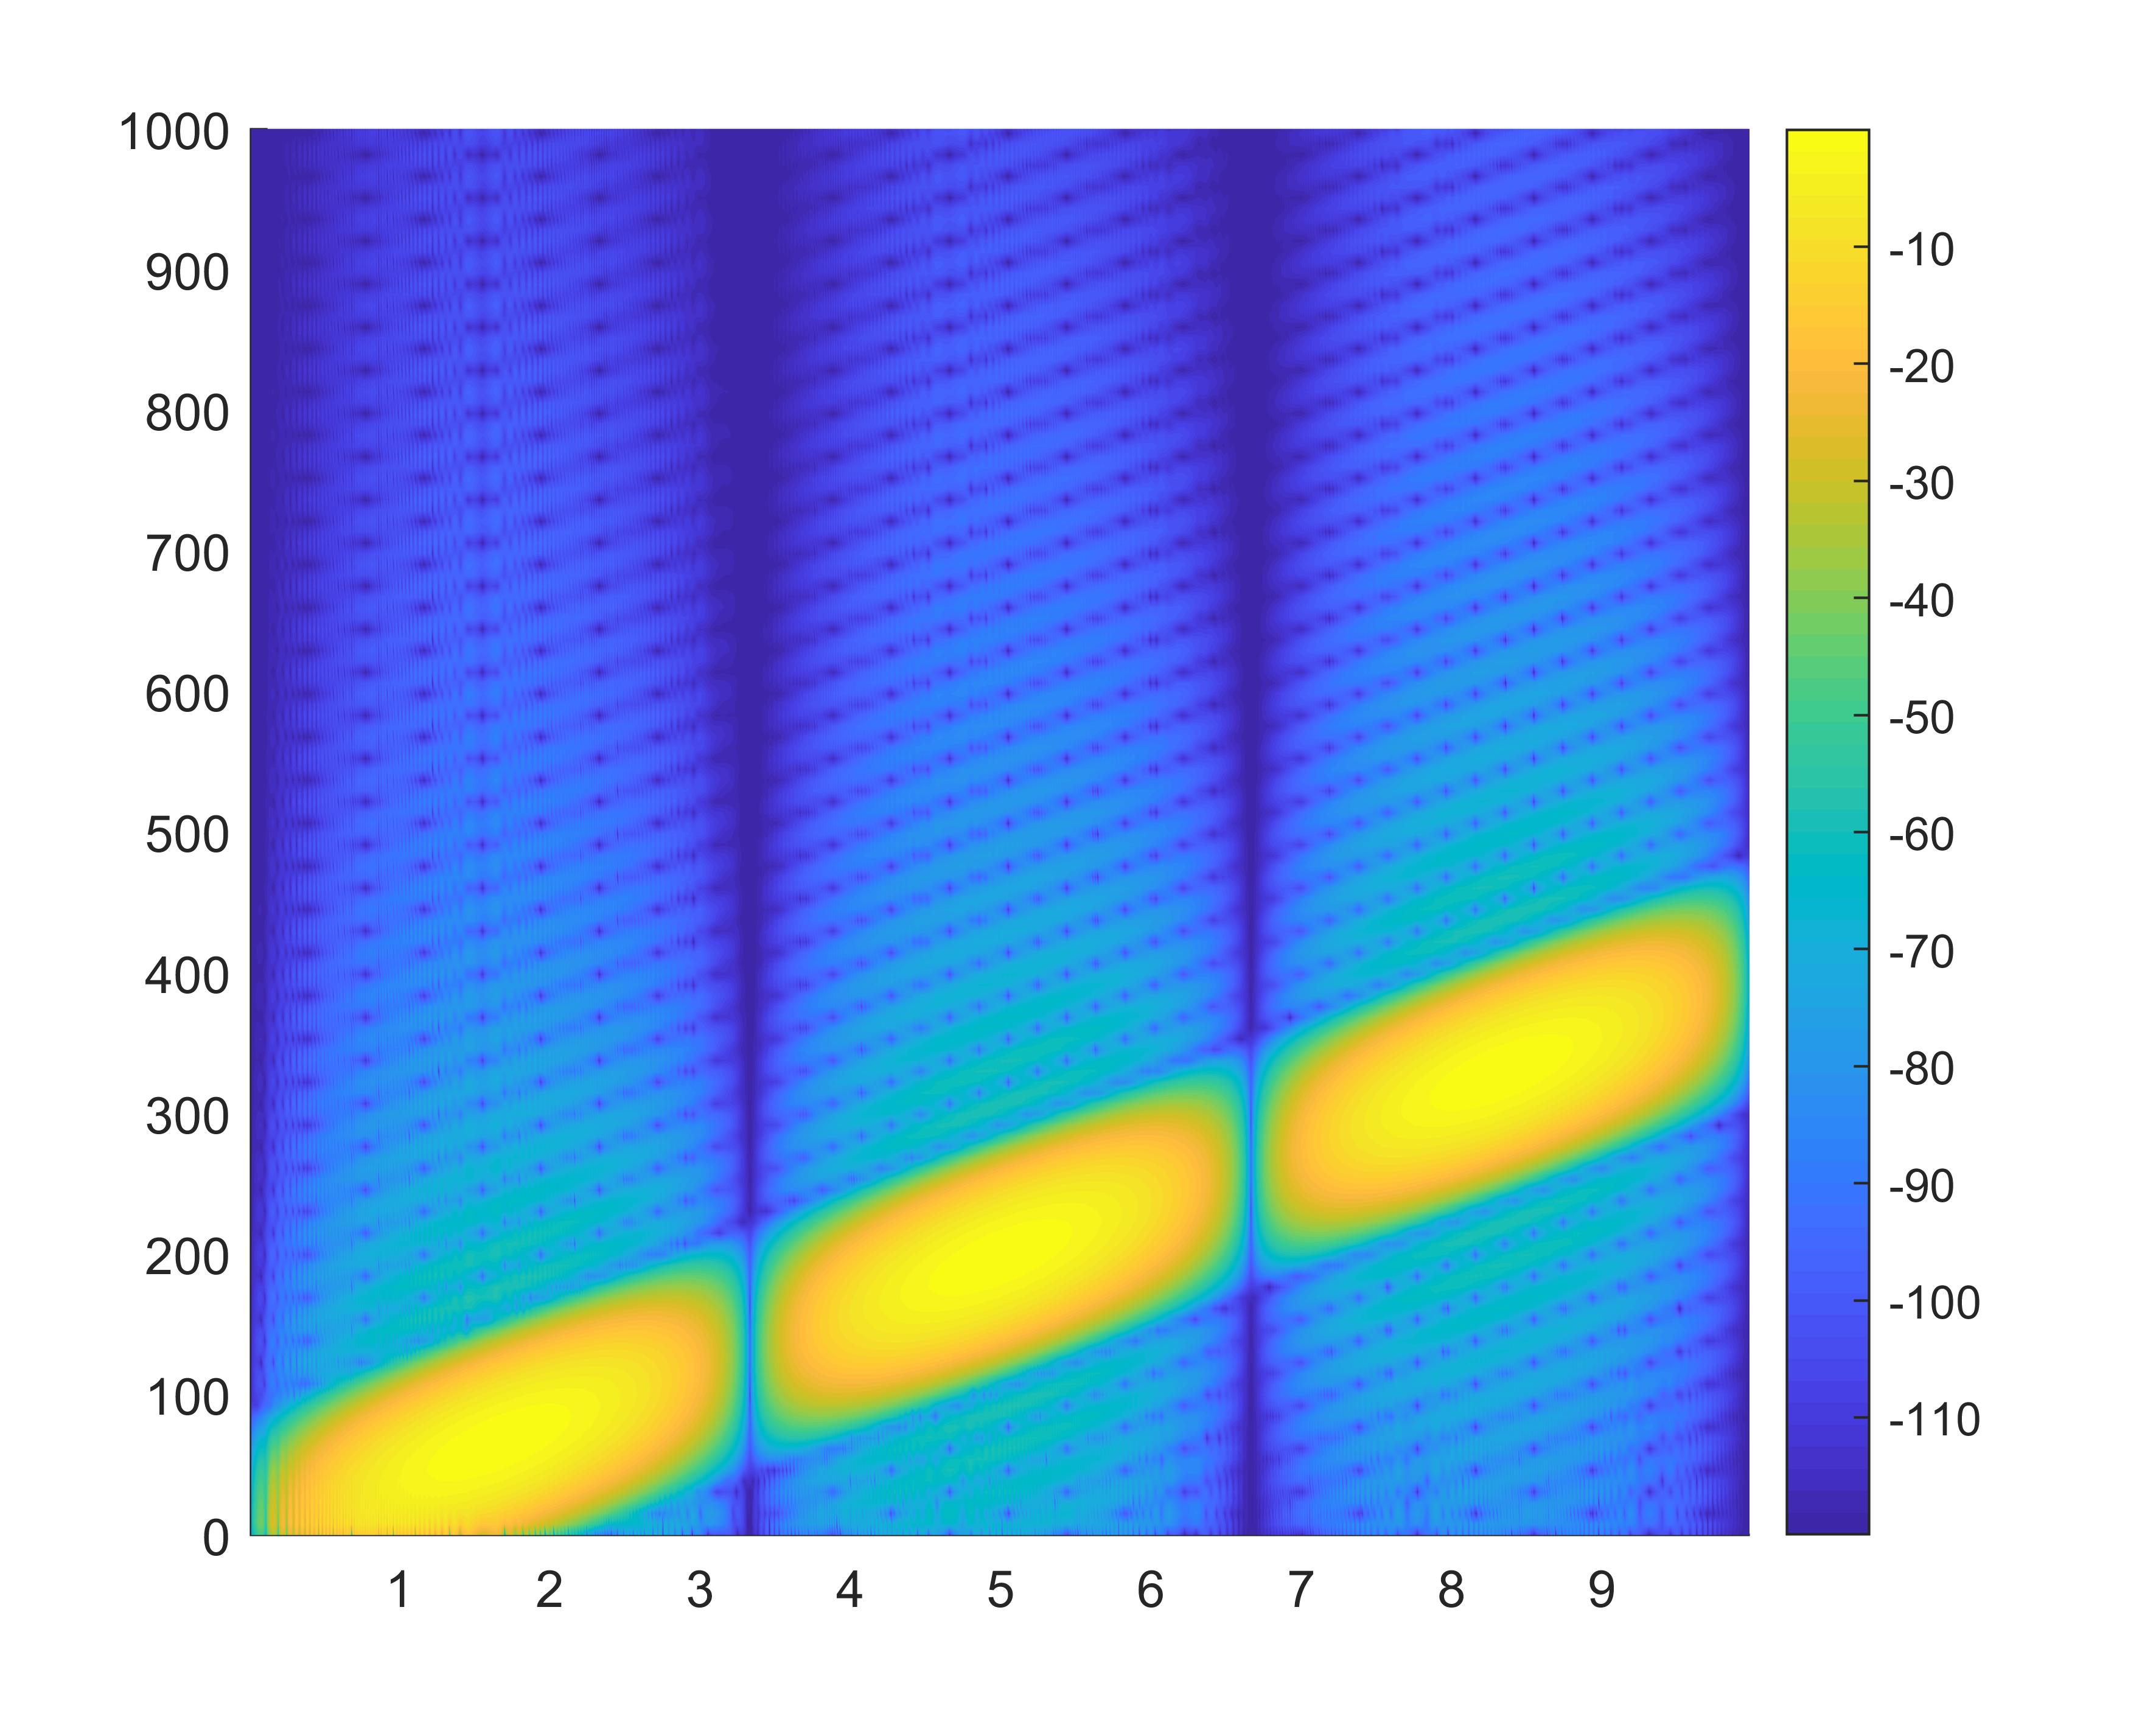
\includegraphics[width=\linewidth]{papers/autotune/sections/fft/stft1024.jpg}   
		\captionof{figure}{1024 Sample Fenster}\label{fig:stft1024}              \\    
		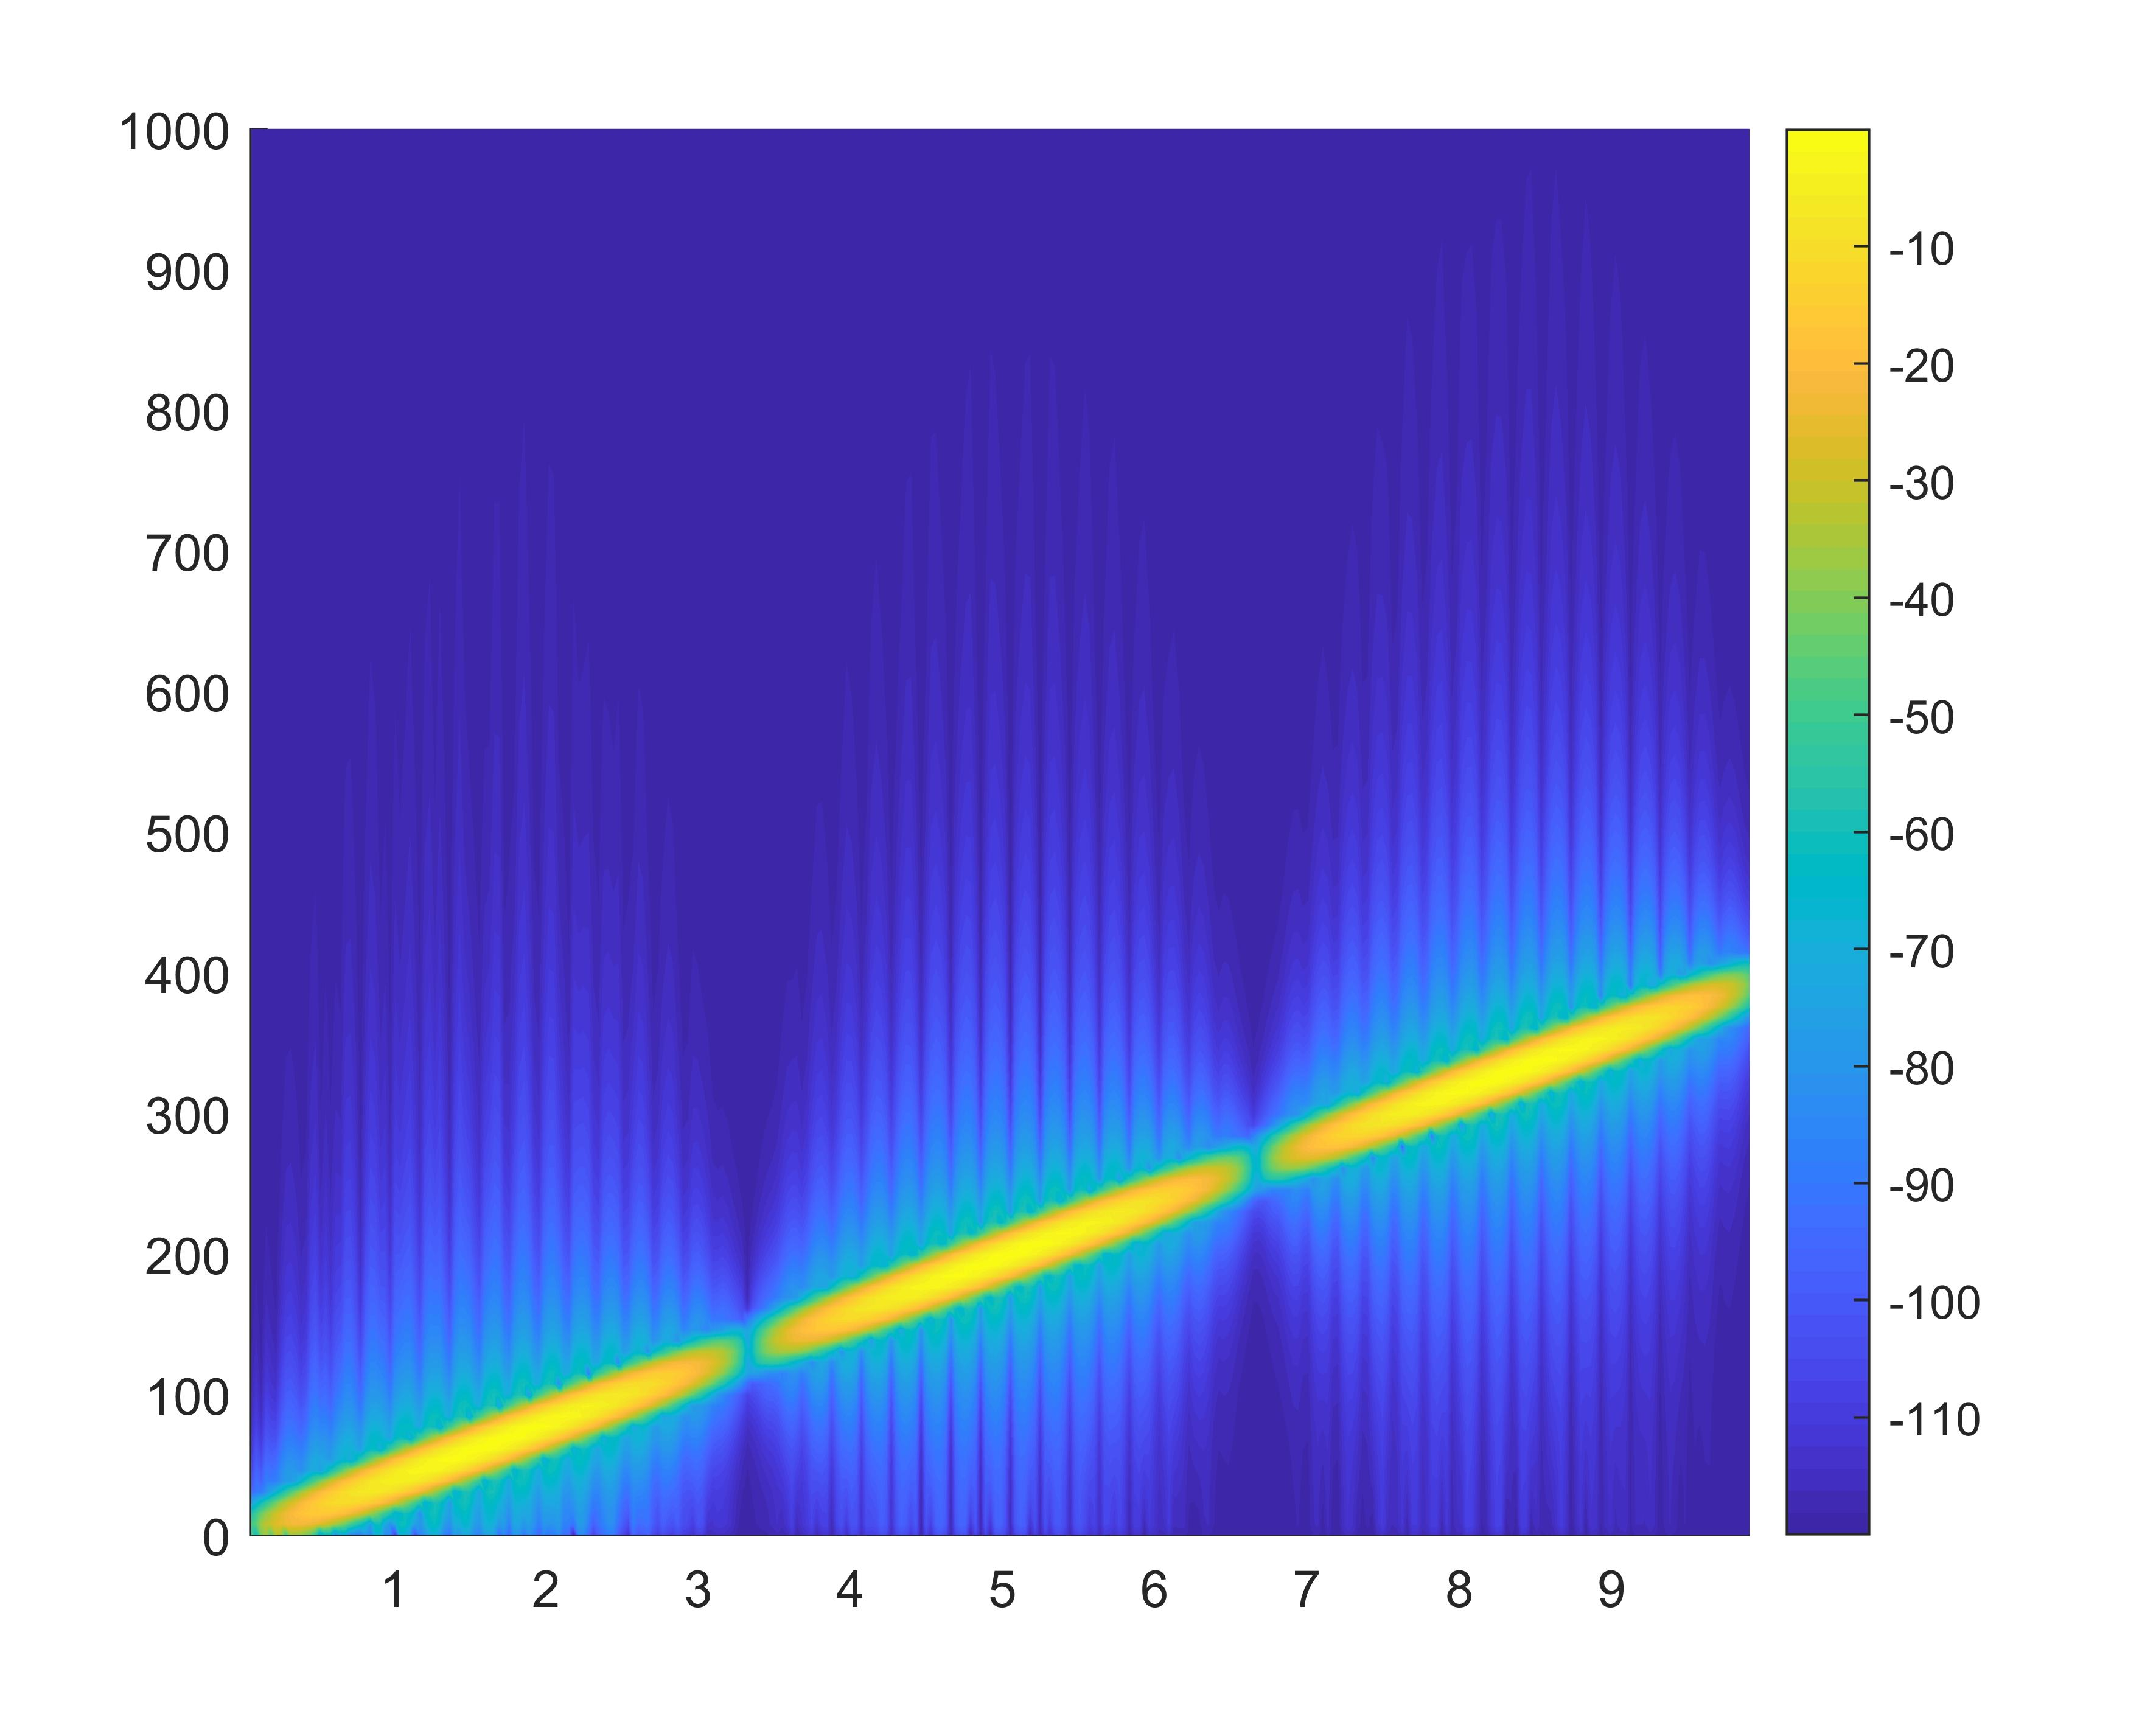
\includegraphics[width=\linewidth]{papers/autotune/sections/fft/stft4096.jpg}
		\captionof{figure}{4096 Sample Fenster}\label{fig:stft4096}
		&   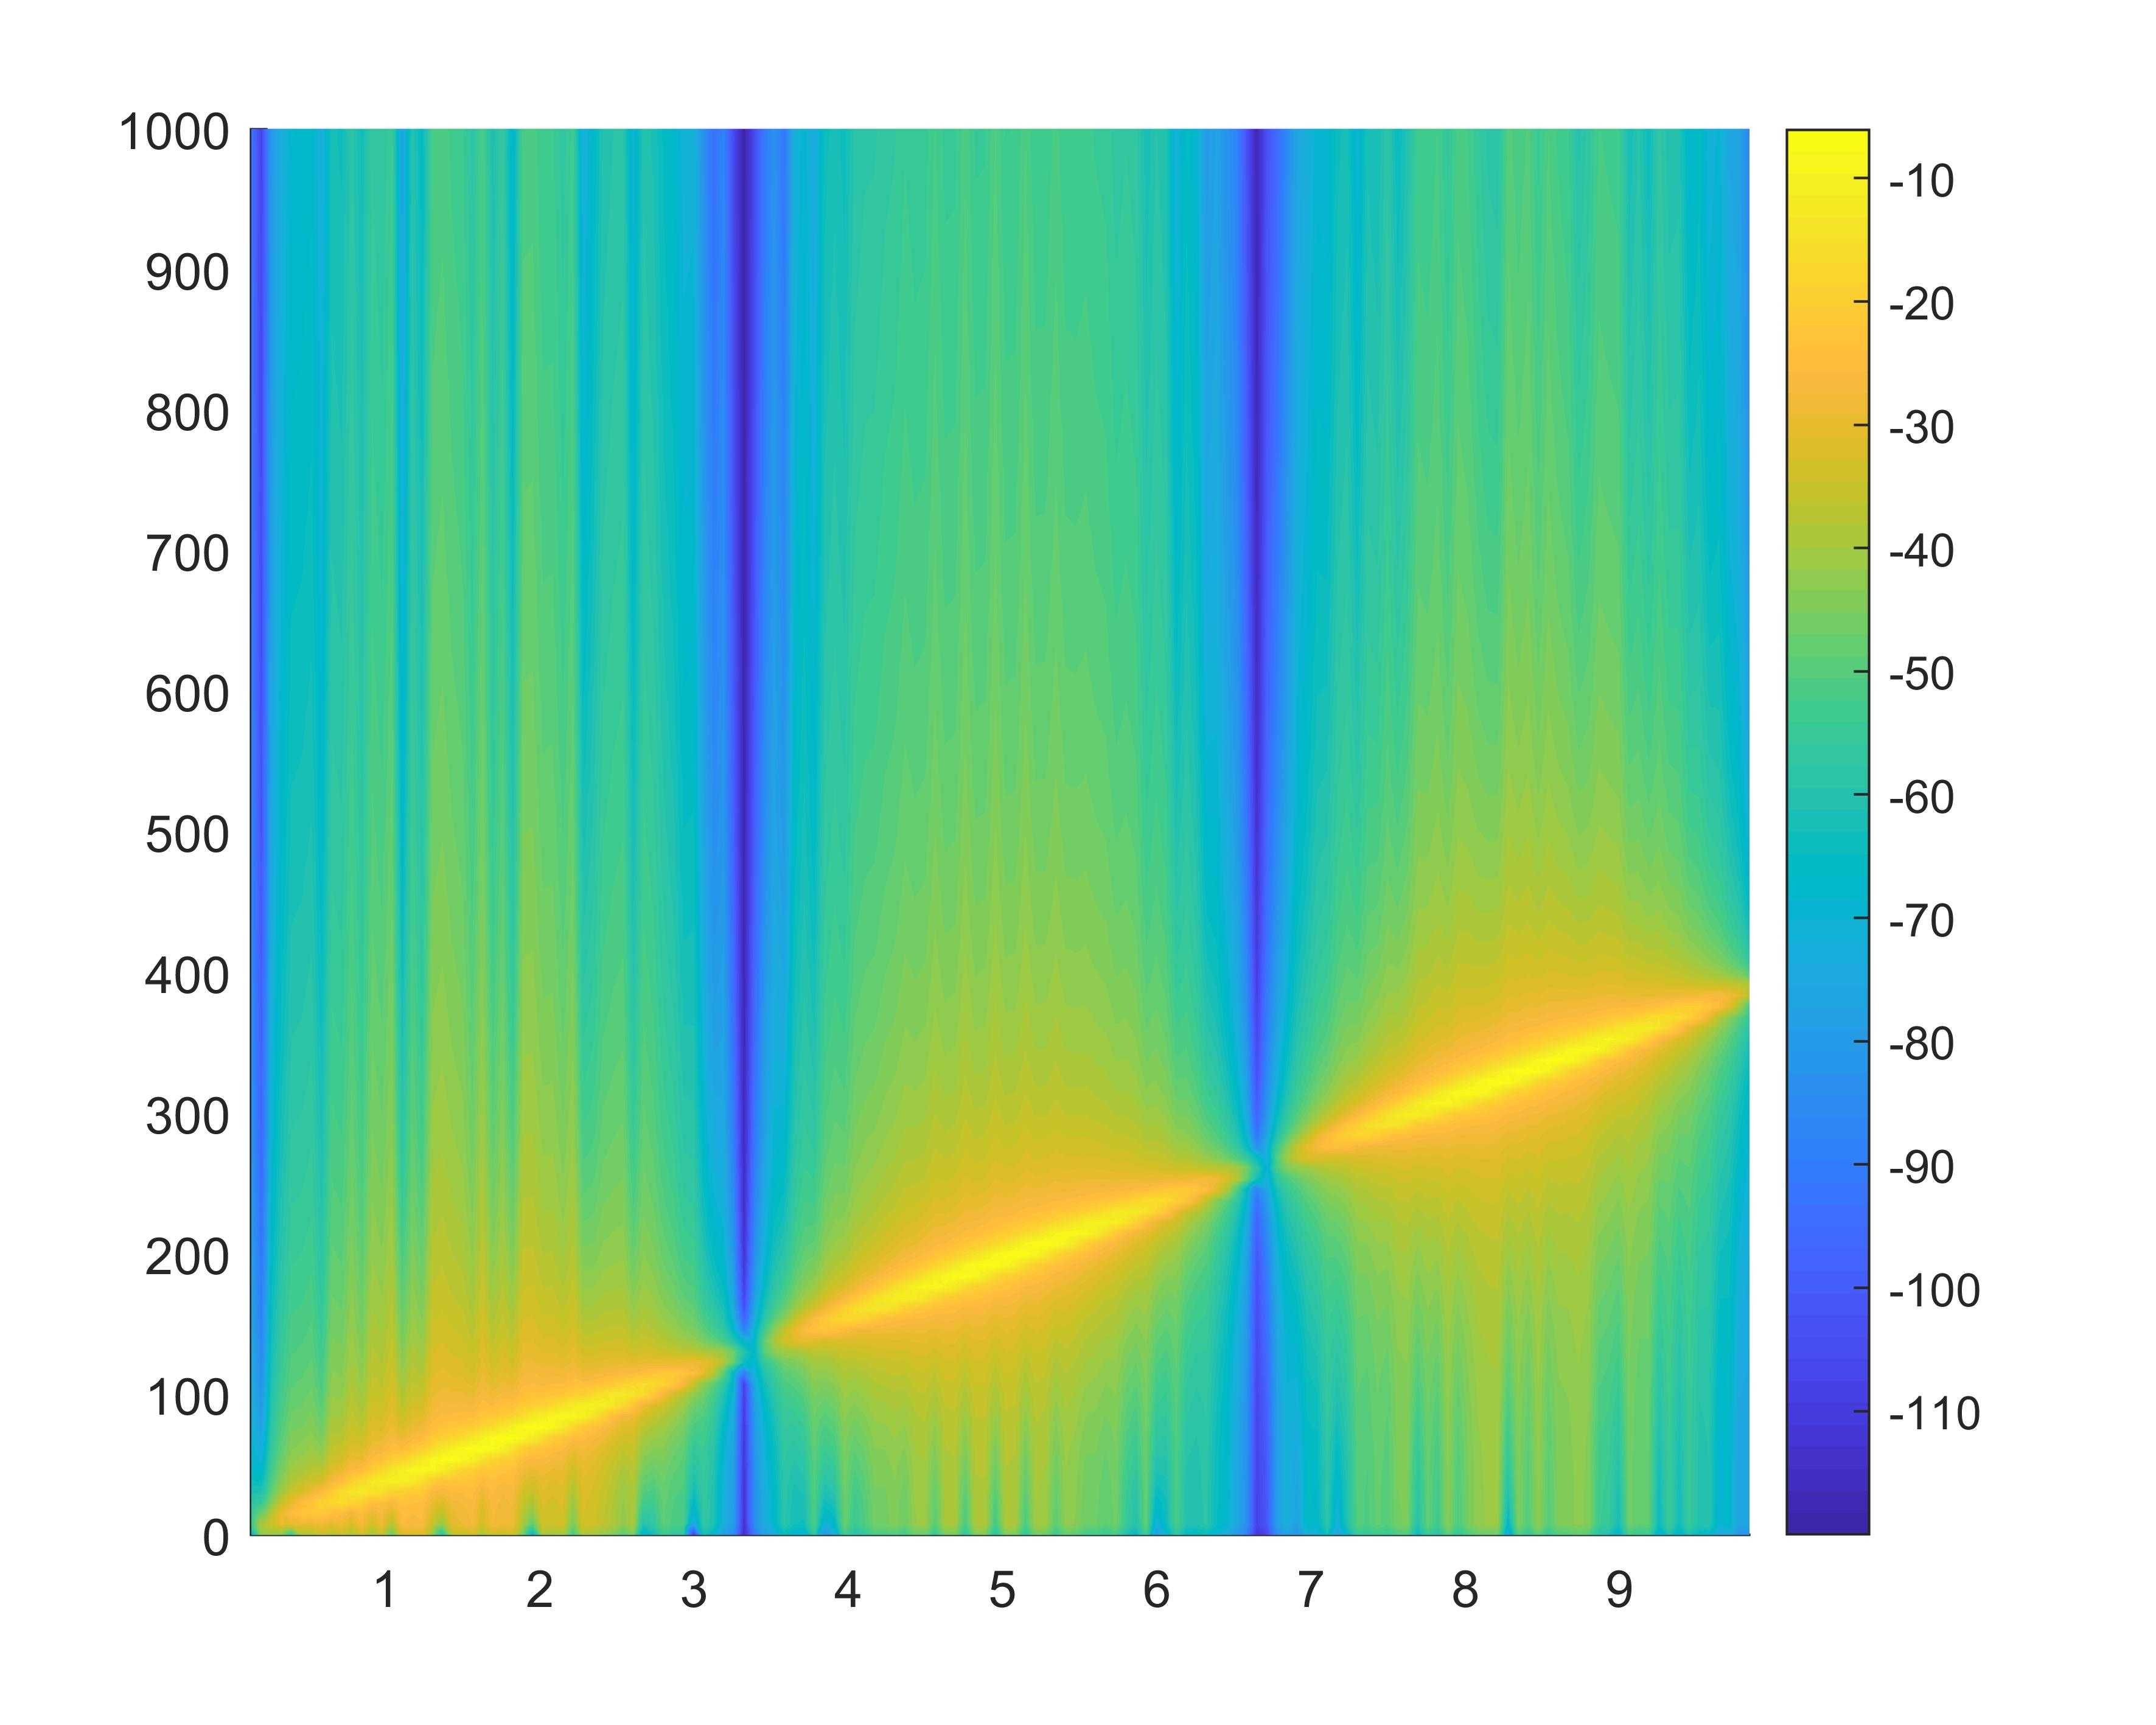
\includegraphics[width=\linewidth]{papers/autotune/sections/fft/stft8192.jpg}   
		\captionof{figure}{8192 Sample Fenster}\label{fig:stft8192}              \\           
	\end{tabularx}
	
	\caption{STFT}
	\label{fig:STFT}
\end{figure}%


Wie man bei der Abbildung \ref{fig:stft256} gleich sieht ist die Streuung noch ernorm. Mann kann nur sehr grob wahrnehmen welche Frequenzen vorhanden sind. Dafür ist die Zeitliche Auflösung sehr gut mit einer scharfen Kante beim Nullpunkt. \\

Betrachtet man nun die Abbildung \ref{fig:stft1024} sind die Frequenzen schon viel deutlicher zu erkennen als bei einem Sampling von 256. Dafür wird in der Zeitlichen Auflösung ein wenig eingebüsst.\\

Das beste Bild ist bei 4096 Samples in der Abbildung \ref{fig:stft4096} zu sehen. Die Zeitliche abgrenzung verschwimmt ein wenig. Dafür ist die Frequenz deutlich ersichtlich.\\

In der Letzten Abbildung \ref{fig:stft8192} ist die zeit so langsam das die tiefen Frequenzen des Modultionssignal wieder einfluss nehmen auf das Spektogramm. Dies verfälscht das Resultat welches dann weniger brauchbar sein kann bei praktischen Auswertungen bei der die Modulationsfrequenz nicht so eine wichtige Rolle spielt.\\






